% minimal_article.tex
%
% Smallest runnable accessible-article example. Compile with:
%
%   lualatex minimal_article.tex
%
% Once this works, see accessible_article.tex for the fully commented
% teaching version with fonts, hyperref configuration, and validator
% notes.

\DocumentMetadata{
  lang        = en-US,
  pdfstandard = ua-2,
  pdfstandard = a-4,
  tagging     = on,
  tagging-setup = {math/setup = mathml-SE},
}

\documentclass{article}

% NOTE: do NOT add \tagpdfsetup{math/alt/use} here. It attaches an /Alt
% string (the raw LaTeX source) to every math Formula tag, and a screen
% reader reads that /Alt *instead of* descending into the generated
% MathML -- so it silences a Blackboard Ally false positive at the cost
% of hiding the real math semantics from screen readers. The MathML
% (math/setup=mathml-SE, set in \DocumentMetadata) is what carries the
% accessible math. See VALIDATION.md.

\usepackage{graphicx}

\title{A minimal accessible article}
\author{Your name}
\date{\today}

\begin{document}

\maketitle

\section{Hello, accessible world}

Compiled with LuaLaTeX. Tagging is on; math is captured as MathML:
\(E = mc^2\). Every image needs an alt description, separate from the
visible caption.

\begin{figure}[ht]
  \centering
  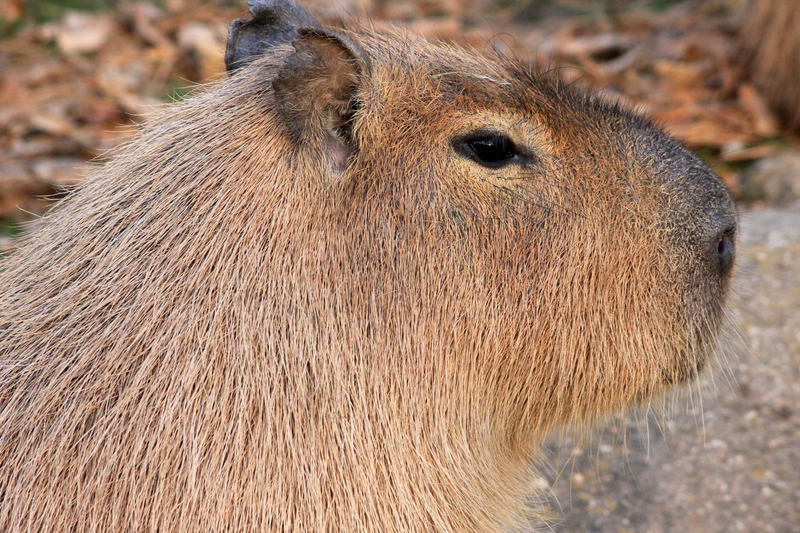
\includegraphics[height=4cm, alt={A capybara's head facing left}]{capybara.jpg}
  \caption{A capybara, used here as a non-decorative illustration.}
\end{figure}

\section{One accessible table}

\tagpdfsetup{table/header-rows = {1}}
\begin{tabular}{lr}
  \textbf{Item} & \textbf{Count} \\
  Apples        & 3              \\
  Oranges       & 5              \\
\end{tabular}

\end{document}
